\documentclass{beamer}
\usepackage[utf8]{inputenc}

\usetheme{Madrid}
\usecolortheme{default}
\usepackage{amsmath,amssymb,amsfonts,amsthm}
\usepackage{txfonts}
\usepackage{tkz-euclide}
\usepackage{listings}
\usepackage{adjustbox}
\usepackage{array}
\usepackage{tabularx}
\usepackage{gvv}
\usepackage{lmodern}
\usepackage{circuitikz}
\usepackage{tikz}
\usepackage{graphicx}

\setbeamertemplate{page number in head/foot}[totalframenumber]

\usepackage{tcolorbox}
\tcbuselibrary{minted,breakable,xparse,skins}



\definecolor{bg}{gray}{0.95}
\DeclareTCBListing{mintedbox}{O{}m!O{}}{%
  breakable=true,
  listing engine=minted,
  listing only,
  minted language=#2,
  minted style=default,
  minted options={%
    linenos,
    gobble=0,
    breaklines=true,
    breakafter=,,
    fontsize=\small,
    numbersep=8pt,
    #1},
  boxsep=0pt,
  left skip=0pt,
  right skip=0pt,
  left=25pt,
  right=0pt,
  top=3pt,
  bottom=3pt,
  arc=5pt,
  leftrule=0pt,
  rightrule=0pt,
  bottomrule=2pt,
  toprule=2pt,
  colback=bg,
  colframe=orange!70,
  enhanced,
  overlay={%
    \begin{tcbclipinterior}
    \fill[orange!20!white] (frame.south west) rectangle ([xshift=20pt]frame.north west);
    \end{tcbclipinterior}},
  #3,
}
\lstset{
    language=C,
    basicstyle=\ttfamily\small,
    keywordstyle=\color{blue},
    stringstyle=\color{orange},
    commentstyle=\color{green!60!black},
    numbers=left,
    numberstyle=\tiny\color{gray},
    breaklines=true,
    showstringspaces=false,
}
%------------------------------------------------------------
%This block of code defines the information to appear in the
%Title page
\title %optional
{2.4.22}
\date{August, 2025}
%\subtitle{A short story}

\author % (optional)
{INDHIRESH S - EE25BTECH11027}



\begin{document}


\frame{\titlepage}
\begin{frame}{Question}
 Find the equation of a plane which bisects perpendicularly the line joining the points $A(2, 3, 4)$ and $B(4, 5, 8)$ at right angles.\\
\end{frame}
\begin{frame}{allowframebreaks}
\frametitle{Equation}

    \centering
    
    \label{tab:parameters}
  Let,
\begin{align}
    \Vec{A}=\myvec{2\\3\\4}\;\;and\;\;\Vec{B}=\myvec{4\\5\\8}
\end{align}
   
\end{frame}


\begin{frame}{Theoretical Solution}
Given that the plane is a perpendicular bisector to the line joining points A and B. Since it is a perpendicular bisector to the line joining points A and B , the midpoint of the line joining points A and B lies on the plane.\\
Let the midpoint of points \textbf{A} and \textbf{B} be \textbf{X}. Then
\begin{align}
||\Vec{X}-\Vec{A}||^2=||\Vec{X}-\Vec{B}||^2
\end{align}
\begin{align}
    ||\Vec{X}||^2+||\Vec{A}||^2-2||\Vec{X}||\;||\Vec{A}||= ||\Vec{X}||^2+||\Vec{B}||^2-2||\Vec{X}||\;||\Vec{B}||
\end{align}
\begin{align}
    ||\Vec{A}||^2-2||\Vec{X}||\;||\Vec{A}||=||\Vec{B}||^2-2||\Vec{X}||\;||\Vec{B}||
\end{align}

\begin{align}
   ||\Vec{A}||^2-||\Vec{B}||^2=2\Vec{X^T}\Vec{A}-2\Vec{X^T}\Vec{B}
\end{align}
\begin{align}
    ||\Vec{A}||^2-||\Vec{B}||^2=2\Vec{X^T}(\Vec{A}-\Vec{B})
\end{align}
which can be written as :
\begin{align}
    ||\Vec{A}||^2-||\Vec{B}||^2=2(\Vec{A}-\Vec{B})^T\Vec{X}
\end{align}



\end{frame}
\begin{frame}
\frametitle{Theoretical Solution}
\begin{align}
 (\Vec{A}-\Vec{B})^T\Vec{X}=\frac{||\Vec{A}||^2-||\Vec{B}||^2}{2}
\end{align}
Now,
\begin{align}
    \Vec{A}-\Vec{B}=\myvec{2\\3\\4}-\myvec{4\\5\\8}
\end{align}
\begin{align}
   \Vec{A}-\Vec{B}=\myvec{-2\\-2\\-4}
\end{align}
And
\begin{align}
     ||\Vec{A}||=\sqrt{\Vec{A^T}\Vec{A}}
\end{align}
\begin{align}
    ||\Vec{A}||=\sqrt{2(2)+3(3)+4(4)}
\end{align}
\end{frame}


\begin{frame}
\frametitle{Theoretical Solution}

\begin{align}
    ||\Vec{A}||=\sqrt{29}
\end{align}

\begin{align}
     ||\Vec{B}||=\sqrt{\Vec{B^T}\Vec{B}}
\end{align}
\begin{align}
     ||\Vec{B}||=\sqrt{4(4)+5(5)+8(8)}
\end{align}
\begin{align}
    ||\Vec{B}||=\sqrt{105}
\end{align}
Now substituting the respective value in Eq.8:
\begin{align}
	\myvec{-2&-2&-4}\Vec{X}=\frac{29-105}{2}
\end{align}



\end{frame}
\begin{frame}
\frametitle{Theoretical Solution}


\begin{align}
	\myvec{1&1&2}\Vec{X}=19
\end{align}
Hence the equation of the plane is given by:
\begin{align}
	\myvec{1&1&2}\Vec{X}=19
\end{align}


\end{frame}





\begin{frame}[fragile]
    \frametitle{C Code - Midpoint formula }

    \begin{lstlisting}
#include <stdio.h>

void midpoint(double A[3], double B[3], double M[3]) {
    M[0] = (A[0] + B[0]) / 2.0;
    M[1] = (A[1] + B[1]) / 2.0;
    M[2] = (A[2] + B[2]) / 2.0;
}

void normal(double A[3], double B[3], double N[3]) {
    N[0] = B[0] - A[0];
    N[1] = B[1] - A[1];
    N[2] = B[2] - A[2];
}

// Compute plane constant: d = -(N · M)
double plane_constant(double N[3], double M[3]) {
    return -(N[0]*M[0] + N[1]*M[1] + N[2]*M[2]);
}


    \end{lstlisting}
\end{frame}


\begin{frame}[fragile]
    \frametitle{Python Code}
    \begin{lstlisting}
import ctypes
import numpy as np
import matplotlib.pyplot as plt

# Load compiled C library
lib = ctypes.CDLL("./libgeometry.so")   # use "geometry.dll" on Windows

# Define argument and return types
lib.midpoint.argtypes = [np.ctypeslib.ndpointer(dtype=np.double, ndim=1, shape=3),
                         np.ctypeslib.ndpointer(dtype=np.double, ndim=1, shape=3),
                         np.ctypeslib.ndpointer(dtype=np.double, ndim=1, shape=3)]









    \end{lstlisting}
\end{frame}

\begin{frame}[fragile]
    \frametitle{Python Code}
    \begin{lstlisting}
lib.normal.argtypes = [np.ctypeslib.ndpointer(dtype=np.double, ndim=1, shape=3),
                       np.ctypeslib.ndpointer(dtype=np.double, ndim=1, shape=3),
                       np.ctypeslib.ndpointer(dtype=np.double, ndim=1, shape=3)]

lib.plane_constant.argtypes = [np.ctypeslib.ndpointer(dtype=np.double, ndim=1, shape=3),
                               np.ctypeslib.ndpointer(dtype=np.double, ndim=1, shape=3)]
lib.plane_constant.restype = ctypes.c_double

# Input points
A = np.array([2.0, 3.0, 4.0], dtype=np.double)
B = np.array([4.0, 5.0, 8.0], dtype=np.double)
M = np.zeros(3, dtype=np.double)
N = np.zeros(3, dtype=np.double)


    \end{lstlisting}
\end{frame}

\begin{frame}[fragile]
    \frametitle{Python Code}

    \begin{lstlisting}
# Call C functions
lib.midpoint(A, B, M)
lib.normal(A, B, N)
d = lib.plane_constant(N, M)

# Plane equation function
def plane_z(x, y):
    return (-N[0] * x - N[1] * y - d) / N[2]

# Create small plane patch around M
span = 1.5
xx, yy = np.meshgrid(
    np.linspace(M[0] - span, M[0] + span, 10),
    np.linspace(M[1] - span, M[1] + span, 10)
)
zz = plane_z(xx, yy)





    \end{lstlisting}
\end{frame}
\begin{frame}[fragile]
    \frametitle{Python Code}

    \begin{lstlisting}
# --- Plotting ---
fig = plt.figure()
ax = fig.add_subplot(111, projection='3d')

# Mark and label points
ax.scatter(*A, color='red', s=100)
ax.text(A[0], A[1], A[2], "A(2,3,4)", color='red')

ax.scatter(*B, color='green', s=100)
ax.text(B[0], B[1], B[2], "B(4,5,8)", color='green')

ax.scatter(*M, color='purple', s=200, marker='*')
ax.text(M[0], M[1], M[2], "M(3,4,6)", color='purple')

# Line AB
ax.plot([A[0], B[0]], [A[1], B[1]], [A[2], B[2]],
        color='blue', label="Line AB")



    \end{lstlisting}
\end{frame}
\begin{frame}[fragile]
    \frametitle{Python Code}

    \begin{lstlisting}


# Plane patch
ax.plot_surface(xx, yy, zz, alpha=0.4, color='cyan')

# Labels and title
ax.set_xlabel("X-axis")
ax.set_ylabel("Y-axis")
ax.set_zlabel("Z-axis")
ax.set_title("Required Plane")
ax.legend()
plt.savefig("/media/indhiresh-s/New Volume/Matrix/ee1030-2025/ee25btech11027/MATGEO/2.4.22/figs/figure1.png")
plt.show()


    \end{lstlisting}
\end{frame}




\begin{frame}{Plot}
    \begin{center}
        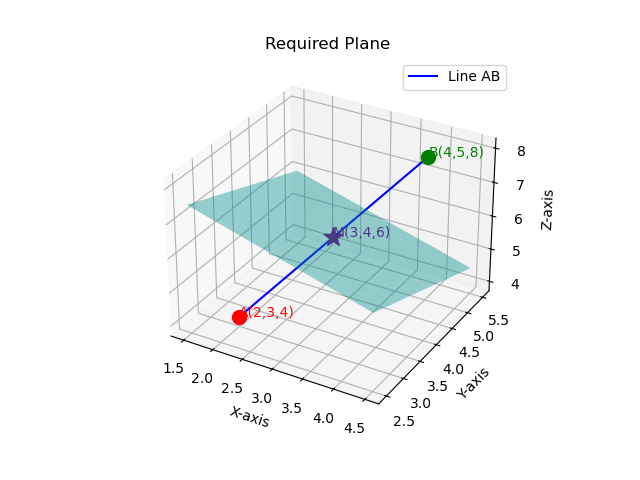
\includegraphics[width=\columnwidth, height=0.8\textheight, keepaspectratio]{figs/figure1.png}
    \end{center}
\end{frame}




\end{document}
